
%% bare_jrnl.tex
%% V1.4b
%% 2015/08/26
%% by Michael Shell
%% see http://www.michaelshell.org/
%% for current contact information.
%%
%% This is a skeleton file demonstrating the use of IEEEtran.cls
%% (requires IEEEtran.cls version 1.8b or later) with an IEEE
%% journal paper.
%%
%% Support sites:
%% http://www.michaelshell.org/tex/ieeetran/
%% http://www.ctan.org/pkg/ieeetran
%% and
%% http://www.ieee.org/

%%*************************************************************************
%% Legal Notice:
%% This code is offered as-is without any warranty either expressed or
%% implied; without even the implied warranty of MERCHANTABILITY or
%% FITNESS FOR A PARTICULAR PURPOSE! 
%% User assumes all risk.
%% In no event shall the IEEE or any contributor to this code be liable for
%% any damages or losses, including, but not limited to, incidental,
%% consequential, or any other damages, resulting from the use or misuse
%% of any information contained here.
%%
%% All comments are the opinions of their respective authors and are not
%% necessarily endorsed by the IEEE.
%%
%% This work is distributed under the LaTeX Project Public License (LPPL)
%% ( http://www.latex-project.org/ ) version 1.3, and may be freely used,
%% distributed and modified. A copy of the LPPL, version 1.3, is included
%% in the base LaTeX documentation of all distributions of LaTeX released
%% 2003/12/01 or later.
%% Retain all contribution notices and credits.
%% ** Modified files should be clearly indicated as such, including  **
%% ** renaming them and changing author support contact information. **
%%*************************************************************************


% *** Authors should verify (and, if needed, correct) their LaTeX system  ***
% *** with the testflow diagnostic prior to trusting their LaTeX platform ***
% *** with production work. The IEEE's font choices and paper sizes can   ***
% *** trigger bugs that do not appear when using other class files.       ***                          ***
% The testflow support page is at:
% http://www.michaelshell.org/tex/testflow/



\documentclass[journal]{IEEEtran}
%
% If IEEEtran.cls has not been installed into the LaTeX system files,
% manually specify the path to it like:
% \documentclass[journal]{../sty/IEEEtran}





% Some very useful LaTeX packages include:
% (uncomment the ones you want to load)


% *** MISC UTILITY PACKAGES ***
%
%\usepackage{ifpdf}
% Heiko Oberdiek's ifpdf.sty is very useful if you need conditional
% compilation based on whether the output is pdf or dvi.
% usage:
% \ifpdf
%   % pdf code
% \else
%   % dvi code
% \fi
% The latest version of ifpdf.sty can be obtained from:
% http://www.ctan.org/pkg/ifpdf
% Also, note that IEEEtran.cls V1.7 and later provides a builtin
% \ifCLASSINFOpdf conditional that works the same way.
% When switching from latex to pdflatex and vice-versa, the compiler may
% have to be run twice to clear warning/error messages.






% *** CITATION PACKAGES ***
%
%\usepackage{cite}
% cite.sty was written by Donald Arseneau
% V1.6 and later of IEEEtran pre-defines the format of the cite.sty package
% \cite{} output to follow that of the IEEE. Loading the cite package will
% result in citation numbers being automatically sorted and properly
% "compressed/ranged". e.g., [1], [9], [2], [7], [5], [6] without using
% cite.sty will become [1], [2], [5]--[7], [9] using cite.sty. cite.sty's
% \cite will automatically add leading space, if needed. Use cite.sty's
% noadjust option (cite.sty V3.8 and later) if you want to turn this off
% such as if a citation ever needs to be enclosed in parenthesis.
% cite.sty is already installed on most LaTeX systems. Be sure and use
% version 5.0 (2009-03-20) and later if using hyperref.sty.
% The latest version can be obtained at:
% http://www.ctan.org/pkg/cite
% The documentation is contained in the cite.sty file itself.






% *** GRAPHICS RELATED PACKAGES ***
%
\ifCLASSINFOpdf
  % \usepackage[pdftex]{graphicx}
  % declare the path(s) where your graphic files are
  % \graphicspath{{../pdf/}{../jpeg/}}
  % and their extensions so you won't have to specify these with
  % every instance of \includegraphics
  % \DeclareGraphicsExtensions{.pdf,.jpeg,.png}
\else
  % or other class option (dvipsone, dvipdf, if not using dvips). graphicx
  % will default to the driver specified in the system graphics.cfg if no
  % driver is specified.
  % \usepackage[dvips]{graphicx}
  % declare the path(s) where your graphic files are
  % \graphicspath{{../eps/}}
  % and their extensions so you won't have to specify these with
  % every instance of \includegraphics
  % \DeclareGraphicsExtensions{.eps}
\fi
% graphicx was written by David Carlisle and Sebastian Rahtz. It is
% required if you want graphics, photos, etc. graphicx.sty is already
% installed on most LaTeX systems. The latest version and documentation
% can be obtained at: 
% http://www.ctan.org/pkg/graphicx
% Another good source of documentation is "Using Imported Graphics in
% LaTeX2e" by Keith Reckdahl which can be found at:
% http://www.ctan.org/pkg/epslatex
%
% latex, and pdflatex in dvi mode, support graphics in encapsulated
% postscript (.eps) format. pdflatex in pdf mode supports graphics
% in .pdf, .jpeg, .png and .mps (metapost) formats. Users should ensure
% that all non-photo figures use a vector format (.eps, .pdf, .mps) and
% not a bitmapped formats (.jpeg, .png). The IEEE frowns on bitmapped formats
% which can result in "jaggedy"/blurry rendering of lines and letters as
% well as large increases in file sizes.
%
% You can find documentation about the pdfTeX application at:
% http://www.tug.org/applications/pdftex





% *** MATH PACKAGES ***
%
%\usepackage{amsmath}
% A popular package from the American Mathematical Society that provides
% many useful and powerful commands for dealing with mathematics.
%
% Note that the amsmath package sets \interdisplaylinepenalty to 10000
% thus preventing page breaks from occurring within multiline equations. Use:
%\interdisplaylinepenalty=2500
% after loading amsmath to restore such page breaks as IEEEtran.cls normally
% does. amsmath.sty is already installed on most LaTeX systems. The latest
% version and documentation can be obtained at:
% http://www.ctan.org/pkg/amsmath





% *** SPECIALIZED LIST PACKAGES ***
%
%\usepackage{algorithmic}
% algorithmic.sty was written by Peter Williams and Rogerio Brito.
% This package provides an algorithmic environment fo describing algorithms.
% You can use the algorithmic environment in-text or within a figure
% environment to provide for a floating algorithm. Do NOT use the algorithm
% floating environment provided by algorithm.sty (by the same authors) or
% algorithm2e.sty (by Christophe Fiorio) as the IEEE does not use dedicated
% algorithm float types and packages that provide these will not provide
% correct IEEE style captions. The latest version and documentation of
% algorithmic.sty can be obtained at:
% http://www.ctan.org/pkg/algorithms
% Also of interest may be the (relatively newer and more customizable)
% algorithmicx.sty package by Szasz Janos:
% http://www.ctan.org/pkg/algorithmicx




% *** ALIGNMENT PACKAGES ***
%
%\usepackage{array}
% Frank Mittelbach's and David Carlisle's array.sty patches and improves
% the standard LaTeX2e array and tabular environments to provide better
% appearance and additional user controls. As the default LaTeX2e table
% generation code is lacking to the point of almost being broken with
% respect to the quality of the end results, all users are strongly
% advised to use an enhanced (at the very least that provided by array.sty)
% set of table tools. array.sty is already installed on most systems. The
% latest version and documentation can be obtained at:
% http://www.ctan.org/pkg/array


% IEEEtran contains the IEEEeqnarray family of commands that can be used to
% generate multiline equations as well as matrices, tables, etc., of high
% quality.




% *** SUBFIGURE PACKAGES ***
%\ifCLASSOPTIONcompsoc
%  \usepackage[caption=false,font=normalsize,labelfont=sf,textfont=sf]{subfig}
%\else
%  \usepackage[caption=false,font=footnotesize]{subfig}
%\fi
% subfig.sty, written by Steven Douglas Cochran, is the modern replacement
% for subfigure.sty, the latter of which is no longer maintained and is
% incompatible with some LaTeX packages including fixltx2e. However,
% subfig.sty requires and automatically loads Axel Sommerfeldt's caption.sty
% which will override IEEEtran.cls' handling of captions and this will result
% in non-IEEE style figure/table captions. To prevent this problem, be sure
% and invoke subfig.sty's "caption=false" package option (available since
% subfig.sty version 1.3, 2005/06/28) as this is will preserve IEEEtran.cls
% handling of captions.
% Note that the Computer Society format requires a larger sans serif font
% than the serif footnote size font used in traditional IEEE formatting
% and thus the need to invoke different subfig.sty package options depending
% on whether compsoc mode has been enabled.
%
% The latest version and documentation of subfig.sty can be obtained at:
% http://www.ctan.org/pkg/subfig




% *** FLOAT PACKAGES ***
%
%\usepackage{fixltx2e}
% fixltx2e, the successor to the earlier fix2col.sty, was written by
% Frank Mittelbach and David Carlisle. This package corrects a few problems
% in the LaTeX2e kernel, the most notable of which is that in current
% LaTeX2e releases, the ordering of single and double column floats is not
% guaranteed to be preserved. Thus, an unpatched LaTeX2e can allow a
% single column figure to be placed prior to an earlier double column
% figure.
% Be aware that LaTeX2e kernels dated 2015 and later have fixltx2e.sty's
% corrections already built into the system in which case a warning will
% be issued if an attempt is made to load fixltx2e.sty as it is no longer
% needed.
% The latest version and documentation can be found at:
% http://www.ctan.org/pkg/fixltx2e


%\usepackage{stfloats}
% stfloats.sty was written by Sigitas Tolusis. This package gives LaTeX2e
% the ability to do double column floats at the bottom of the page as well
% as the top. (e.g., "\begin{figure*}[!b]" is not normally possible in
% LaTeX2e). It also provides a command:
%\fnbelowfloat
% to enable the placement of footnotes below bottom floats (the standard
% LaTeX2e kernel puts them above bottom floats). This is an invasive package
% which rewrites many portions of the LaTeX2e float routines. It may not work
% with other packages that modify the LaTeX2e float routines. The latest
% version and documentation can be obtained at:
% http://www.ctan.org/pkg/stfloats
% Do not use the stfloats baselinefloat ability as the IEEE does not allow
% \baselineskip to stretch. Authors submitting work to the IEEE should note
% that the IEEE rarely uses double column equations and that authors should try
% to avoid such use. Do not be tempted to use the cuted.sty or midfloat.sty
% packages (also by Sigitas Tolusis) as the IEEE does not format its papers in
% such ways.
% Do not attempt to use stfloats with fixltx2e as they are incompatible.
% Instead, use Morten Hogholm'a dblfloatfix which combines the features
% of both fixltx2e and stfloats:
%
% \usepackage{dblfloatfix}
% The latest version can be found at:
% http://www.ctan.org/pkg/dblfloatfix




%\ifCLASSOPTIONcaptionsoff
%  \usepackage[nomarkers]{endfloat}
% \let\MYoriglatexcaption\caption
% \renewcommand{\caption}[2][\relax]{\MYoriglatexcaption[#2]{#2}}
%\fi
% endfloat.sty was written by James Darrell McCauley, Jeff Goldberg and 
% Axel Sommerfeldt. This package may be useful when used in conjunction with 
% IEEEtran.cls'  captionsoff option. Some IEEE journals/societies require that
% submissions have lists of figures/tables at the end of the paper and that
% figures/tables without any captions are placed on a page by themselves at
% the end of the document. If needed, the draftcls IEEEtran class option or
% \CLASSINPUTbaselinestretch interface can be used to increase the line
% spacing as well. Be sure and use the nomarkers option of endfloat to
% prevent endfloat from "marking" where the figures would have been placed
% in the text. The two hack lines of code above are a slight modification of
% that suggested by in the endfloat docs (section 8.4.1) to ensure that
% the full captions always appear in the list of figures/tables - even if
% the user used the short optional argument of \caption[]{}.
% IEEE papers do not typically make use of \caption[]'s optional argument,
% so this should not be an issue. A similar trick can be used to disable
% captions of packages such as subfig.sty that lack options to turn off
% the subcaptions:
% For subfig.sty:
% \let\MYorigsubfloat\subfloat
% \renewcommand{\subfloat}[2][\relax]{\MYorigsubfloat[]{#2}}
% However, the above trick will not work if both optional arguments of
% the \subfloat command are used. Furthermore, there needs to be a
% description of each subfigure *somewhere* and endfloat does not add
% subfigure captions to its list of figures. Thus, the best approach is to
% avoid the use of subfigure captions (many IEEE journals avoid them anyway)
% and instead reference/explain all the subfigures within the main caption.
% The latest version of endfloat.sty and its documentation can obtained at:
% http://www.ctan.org/pkg/endfloat
%
% The IEEEtran \ifCLASSOPTIONcaptionsoff conditional can also be used
% later in the document, say, to conditionally put the References on a 
% page by themselves.




% *** PDF, URL AND HYPERLINK PACKAGES ***
%
%\usepackage{url}
% url.sty was written by Donald Arseneau. It provides better support for
% handling and breaking URLs. url.sty is already installed on most LaTeX
% systems. The latest version and documentation can be obtained at:
% http://www.ctan.org/pkg/url
% Basically, \url{my_url_here}.




% *** Do not adjust lengths that control margins, column widths, etc. ***
% *** Do not use packages that alter fonts (such as pslatex).         ***
% There should be no need to do such things with IEEEtran.cls V1.6 and later.
% (Unless specifically asked to do so by the journal or conference you plan
% to submit to, of course. )


% correct bad hyphenation here
\hyphenation{op-tical net-works semi-conduc-tor}

\usepackage[slovene]{babel}
\usepackage[utf8]{inputenc}
\usepackage[T1]{fontenc}
\usepackage{lmodern}

% Te pakete sem jaz sam vključil:
\usepackage{verbatim} % za bločne komentarje
\usepackage{amsfonts} % za številske množice
\usepackage{amsmath} % za krepke simbole
\usepackage{graphicx}

\begin{document}
%
% paper title
% Titles are generally capitalized except for words such as a, an, and, as,
% at, but, by, for, in, nor, of, on, or, the, to and up, which are usually
% not capitalized unless they are the first or last word of the title.
% Linebreaks \\ can be used within to get better formatting as desired.
% Do not put math or special symbols in the title.
\title{Slikovno vodena radioterapija glave in vratu:\\pregled področja}
%
%
% author names and IEEE memberships
% note positions of commas and nonbreaking spaces ( ~ ) LaTeX will not break
% a structure at a ~ so this keeps an author's name from being broken across
% two lines.
% use \thanks{} to gain access to the first footnote area
% a separate \thanks must be used for each paragraph as LaTeX2e's \thanks
% was not built to handle multiple paragraphs
%

\author{Domen~Močnik,~\IEEEmembership{Fakulteta~za~elektrotehniko,~Univerza~v~Ljubljani,~Tržaška~25,~1000~Ljubljana}}% <-this % stops a space

% note the % following the last \IEEEmembership and also \thanks - 
% these prevent an unwanted space from occurring between the last author name
% and the end of the author line. i.e., if you had this:
% 
% \author{....lastname \thanks{...} \thanks{...} }
%                     ^------------^------------^----Do not want these spaces!
%
% a space would be appended to the last name and could cause every name on that
% line to be shifted left slightly. This is one of those "LaTeX things". For
% instance, "\textbf{A} \textbf{B}" will typeset as "A B" not "AB". To get
% "AB" then you have to do: "\textbf{A}\textbf{B}"
% \thanks is no different in this regard, so shield the last } of each \thanks
% that ends a line with a % and do not let a space in before the next \thanks.
% Spaces after \IEEEmembership other than the last one are OK (and needed) as
% you are supposed to have spaces between the names. For what it is worth,
% this is a minor point as most people would not even notice if the said evil
% space somehow managed to creep in.



% The paper headers
%\markboth{Journal of \LaTeX\ Class Files,~Vol.~14, No.~8, August~2015}%
%{Shell \MakeLowercase{\textit{et al.}}: Bare Demo of IEEEtran.cls for IEEE Journals}
% The only time the second header will appear is for the odd numbered pages
% after the title page when using the twoside option.
% 
% *** Note that you probably will NOT want to include the author's ***
% *** name in the headers of peer review papers.                   ***
% You can use \ifCLASSOPTIONpeerreview for conditional compilation here if
% you desire.




% If you want to put a publisher's ID mark on the page you can do it like
% this:
%\IEEEpubid{0000--0000/00\$00.00~\copyright~2015 IEEE}
% Remember, if you use this you must call \IEEEpubidadjcol in the second
% column for its text to clear the IEEEpubid mark.



% use for special paper notices
%\IEEEspecialpapernotice{(Invited Paper)}




% make the title area
\maketitle

% As a general rule, do not put math, special symbols or citations
% in the abstract or keywords.
\begin{abstract}
Naprave v sodobni radioterapiji omogočajo oblikovanje nehomogenih polj intenzitet sevanja, kar ponuja možnost za natančnejše dostavljanje visoke doze sevanja v rakave celice in izboljšano prizanašanje okoliškemu tkivu, ki ga sevanje prav tako poškoduje. V ta namen je potrebna natančna določitev lege anatomskih struktur pacienta v položaju obsevanja iz zajete medicinske slike. V večtedenskem obdobju radioterapije prihaja do krčenja obsevanega tkiva in do sprememb v legi pacienta med obsevanjem, zato je potrebno podatke o legi sproti posodabljati, kar se doseže s poravnavo slike z orisanimi strukturami na aktualno sliko. Poravnava slik se v radioterapiji uporablja tudi za združevanje komplementarnih anatomskih ali funkcionalnih informacij, pridobljenih iz medicinskih slik, zajetih po različnih protokolih, s čimer se izboljša analitske in diagnostične zmožnosti zdravnika. Poročilo zajema pregled nedavnih raziskav poravnave medicinskih slik v radioterapiji glave in vratu ter povzema glavne rezultate.
\end{abstract}

% Note that keywords are not normally used for peerreview papers.
%\begin{IEEEkeywords}
%IEEE, IEEEtran, journal, \LaTeX, paper, template.
%\end{IEEEkeywords}






% For peer review papers, you can put extra information on the cover
% page as needed:
% \ifCLASSOPTIONpeerreview
% \begin{center} \bfseries EDICS Category: 3-BBND \end{center}
% \fi
%
% For peerreview papers, this IEEEtran command inserts a page break and
% creates the second title. It will be ignored for other modes.
\IEEEpeerreviewmaketitle



\section{Uvod}

Celica, obsevana z visokoenergijskim ionizirajočim sevanjem, utrpi poškodbo svojega genskega materiala, s čimer izgubi svoj potencial za nadalnjo delitev in sčasoma odmre. Cilj učinkovite sodobne radioterapije je prenesti čim večjo dozo ionizirajočega sevanja v celice rakavega tkiva, hkrati pa čim bolj zmanjšati sevalno izpostavljenost normalnih celic okoliškega zdravega tkiva \cite{baskar2012}.

Večlistnati kolimator je naprava, ki s preusmerjanjem delcev sevanja iz izvora omogočaj oblikovanje zapletenega radiacijskega polja (prostorske porazdelitve intenzitete sevanja) s strmimi gradienti. Tovrstne naprave torej omogočajo oblikovanje takega radiacijskega polja, da se območje z visoko intenziteto dobro prilega tumorju, za kar pa je potrebno dobro poznati lokacijo tumorja. V ta namen se pred radioterapijo zajame medicinsko CT (računalniška tomografija, angl.~computed tomography) ali MR (magnetna resonanca) sliko pacienta (načrtovalno sliko), na kateri zdravnik oriše bruto volumen tumorja (področje na sliki, za katerega je razvidno, da pripada tumorju), volumen klinične tarče (bruto volumen tumorja skupaj z okolico subkliničnega širjenja bolezni) ter morebitne kritične organe, ki so vitalnega pomena za pacienta in se jim mora sevanje v čim večji meri izogniti. Ker med postopkom slikanja ali radioterapije lahko pride do manjših anatomskih premikov (nekaj mm) zaradi dihanja, požiranja, krčenja mišic, itn., zajema načrtovani volumen radioterapije poleg volumna klinične tarče še dodatno okolico, s katero je zagotovljeno, da je pokrit celoten tumor \cite{burnet2004}. Na podlagi orisanih volumnov računalniški program izračuna optimalno radiacijsko polje za obsevanje. Opisani postopek se imenuje intenzitetno modulirana radioterapija \cite{jaffray2012}.

Celotno zdravljenje pacienta z radioterapijo v območju glave in vratu običajno poteka v več delih (frakcijah) z dnevnimi presledki skozi obdobje več tednov. V tem obdobju lahko pride do večjih sprememb v volumnu anatomskih struktur; med drugim se v povprečju tumor skrči za $70\%$, parotidne žleze za $50\%$, telesna masa se zmanjša za $3\%$ \cite{al-mayah2015}. Nadalje med posameznimi frakcijami radioterapije prihaja do odstopanj v legi pacienta. Zato načrtovalna slika sčasoma ne odraža več natančno aktualnih položajev orisanih volumnov. Sodobne naprave za radioterapijo združujejo tudi CT ali pa CBCT (CT s stožčastim žarkom, angl.~cone beam CT) skenerje, s katerimi je mogoče zajeti sliko pacienta v položaju za obsevanje nekaj trenutkov pred začetkom frakcije (medterapevtska slika), ki natančno odraža aktualni položaj in se lahko uporabi za izboljšanje natančnosti radiacijskega polja. Ročno orisovanje volumnov tumorja in kritičnih struktur je zamudno opravilo, zato se orisovanje opravi zgolj enkrat, na načrtovalni sliki, nato pa se pred vsako frakcijo z avtomatskimi postopki poravna načrtovalno sliko na aktualno medterapevtsko sliko, s čimer se poravna tudi orisane volumne in tako se lahko oblikovanje radiacijskega polja sproti prilagaja trenutni legi anatomskih struktur pacienta. Tovrstna tehnika se imenuje slikovno vodena radioterapija (slika~\ref{diagram}).

V nekaterih primerih sta za načrtovanju radioterapije na voljo tako MR kot tudi CT slika. MR slike imajo v primerjavi s CT slikami veliko boljši kontrast na področju mehkih tkiv in zato pripomorejo k natančnejšemu orisovanju volumnov tumorjev in normalnih tkiv. CT slike so geometrijsko natančne (brez distorzije) in vsebujejo informacijo o elektronski gostoti tkiva. Da bi izrabili prednosti obeh modalitet za načrtovanje radioterapije, je potrebno MR in CT sliko prostorsko poravnati.

Ker je torej od natančnosti slikovne poravnave odvisna tudi natančnost slikovno vodene radioterapije, je smiselno izboljševati natančnost poravnave slik.

\begin{figure} \centering
 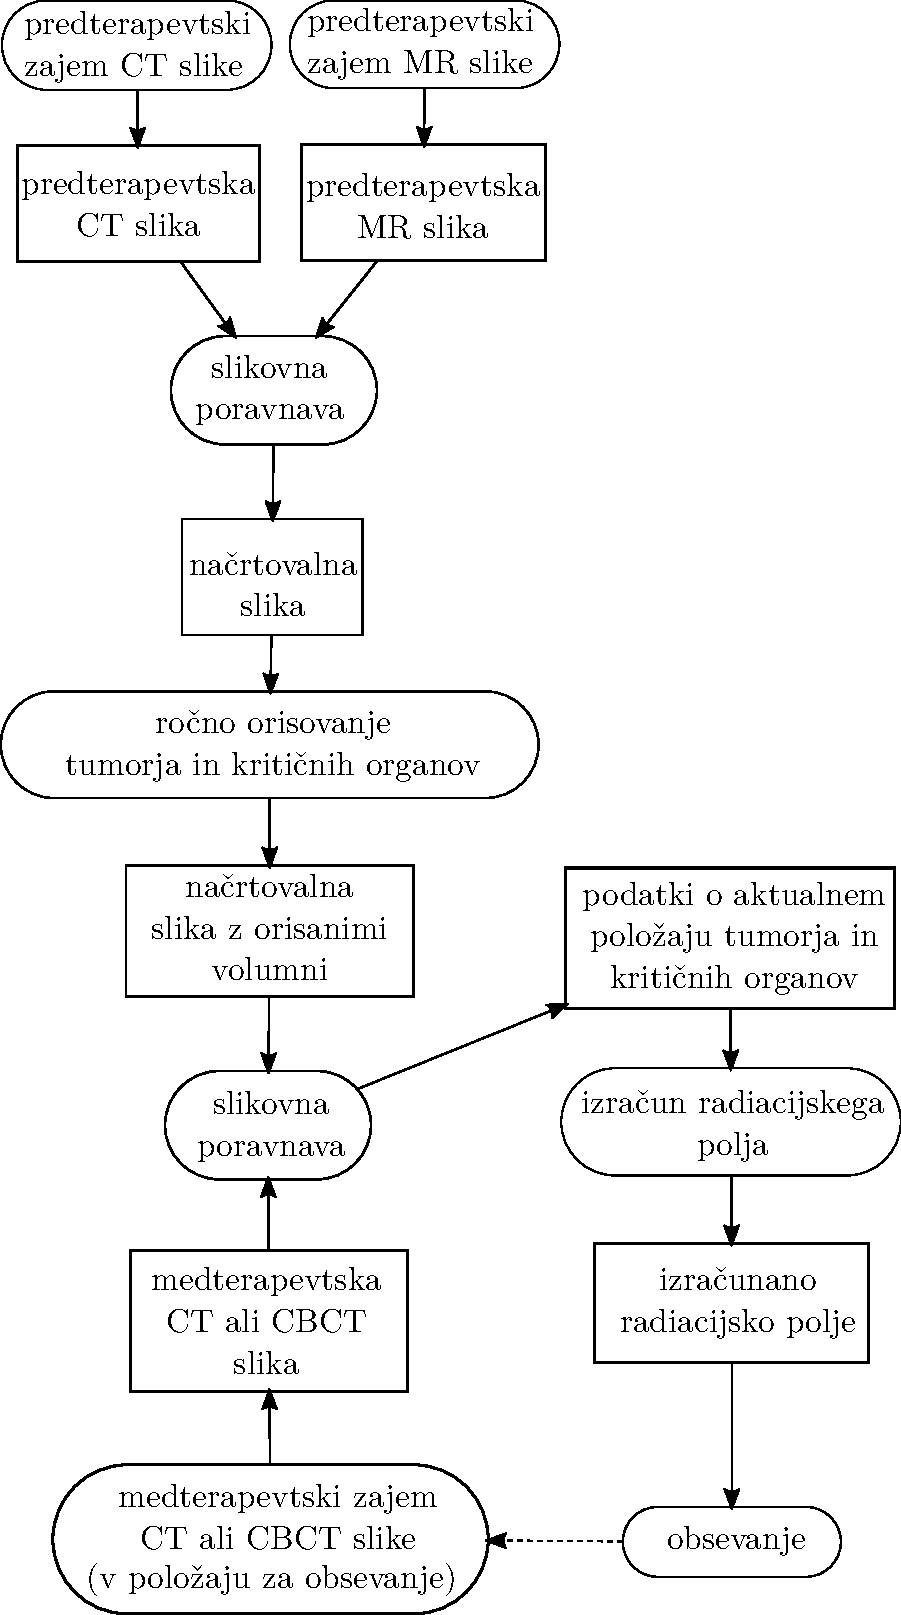
\includegraphics[width=7.5cm]{./diagram.pdf}
 % diagram.pdf: 0x0 pixel, 0dpi, 0.00x0.00 cm, bb=
 \caption{Potek slikovno vodene radioterapije.}
 \label{diagram}
\end{figure}




\section{Postopki za avtomatsko poravnavo medicinskih slik v radioterapiji glave in vratu}


Slikovna poravnava je postopek za iskanje prostorskih preslikav med dvema ali več zajetimi slikami, ki med njimi vzpostavi smiselno anatomsko ali funkcionalno korespondenco. V tem poročilu se bomo omejili na poravnavo dveh slik. Ena izmed njiju se običajno imenuje \emph{izvor} ali \emph{gibljiva slika}, druga pa \emph{tarča} ali \emph{negibna slika}. Gibljiva slika je podana s preslikavo $S\colon\Omega_S\subset\mathbb{R}^2\to\mathbb{R}$, negibna slika pa s $T\colon\Omega_T\subset\mathbb{R}^2\to\mathbb{R}$. $\Omega_S$ in $\Omega_T$ sta slikovni domeni (običajno pravokotni), medtem ko vrednosti preslikav predstavljajo slikovne intenzitete. Cilj registracije je poiskati preslikavo $W\colon\Omega_S\to\Omega_T$, ki kar se da dobro poravna sliki. Preslikavo $W$ običajno zapišemo v obliki
\begin{equation}
 W(\boldsymbol{x}) = \boldsymbol{x} + \boldsymbol{u}(\boldsymbol{x}),
\end{equation}
kjer je $\boldsymbol{u}$ vektorsko polje pomikov.

Algoritem za poravnavo običajno sestoji iz treh ključnih komponent: \emph{deformacijski model}, \emph{kriterijska funkcija} in pa \emph{optimizacijska metoda}. Deformacijski model je predpis, s katerim podamo množico vseh možnih preslikav, med katerimi algoritem potem skuša poiskati optimalno. Če se da to množico parametrizirati s kako podmnožico $\Theta\subset\mathbb{R}^n$, potem rečemo, da je model \emph{$n$-parametričen} ali pa da ima $n$ \emph{prostostnih stopenj}. Kriterijska funkcija je funkcija, ki kvantitativno ovrednoti, kako dobro sta sliki poravnani. Če je model parametriziran z množico $\Theta$, potem se pričakuje, da kriterijska funkcija $f\colon\Theta\to\mathbb{R}$ zavzame svoj minimum pri tistem parametru $\boldsymbol{\theta}\in\Theta$, ki v danem modelu ponuja najboljšo poravnavo slik. Optimizacijska metoda skuša poiskati minimum kriterijske funkcije in je računsko najbolj zahteven del algoritma.

\subsection{Vrednotenje kakovosti poravnave slik}

Pri kvantitativnem vrednotenju kakovosti avtomatske poravnave slik veliko težavo predstavlja nepoznavanje resnične preslikave, zaradi česar je, razen v sintetičnih primerih, nemogoče primerjati izračunano in resnično preslikavo. Zato se metode za vrednotenje v praksi zanašajo na referenčne podatke, ki jih ročno vnesejo strokovnjaki.

Kvantitativno vrednotenje kakovosti poravnave slik v praksi poteka tako, da strokovnjak na slikah (na izvoru in na tarči)
\begin{enumerate}
\item označi $n$ parov oslonilnih točk $(\lambda_i,\kappa_i)\in\Omega_S\times\Omega_T$, ($i=1,\dots,n$), tako da točki iz para $(\lambda_i, \kappa_i)$ označujeta isto anatomsko lokacijo, vidno na obeh slikah, nato pa se izračunajo statistike, ki vključujejo evklidske razdalje $d_i=\|W(\boldsymbol{\lambda}_i)-\boldsymbol{\kappa}_i\|_2$, recimo njihovo povprečje in standardna deviacija, minimum, maksimum idr.
\item oriše območji zanimanja $A\subset\Omega_S$, $B\subset\Omega_T$, recimo katerega od organov ali pa tumor, nato pa se izračuna mere, kot so Dice, Hausdorffova razdalja idr., ki vrednotijo prekrivanje originalnega področja $B$ in preslikanega območja $W(A)$.
\end{enumerate}

V nadaljevanju sledi pregled ovrednotenih postopkov za poravnavo slik, ki se uporabljajo v slikovno vodeni radioterapiji glave in vratu.

\subsection{Poravnave CT na CT}

V delu \cite{hardcastle2012} so avtorji ocenjevali uspešnost slikovne poravnave, kjer so bile tako načrtovalne kot tudi medterapevtske slike zajete s spiralnim CT skenerjem. Avtorji so imeli na voljo 22 parov slik različnih pacientov z neoplazmami na področju glave in vratu. Na slikah je izkušeni zdravnik orisal bruto volumen tumorja ter naslednje kritične organe: hrbtenjačo, možgansko deblo in parotidni žlezi. Za slikovno poravnavo so uporabili večmrežno metodo Demons \cite{vercauteren2009}, ki išče deformacijsko polje kot rešitev difuzijske enačbe, in pa metodo za poravnavo na podlagi perečih značilnic (angl.~salient-feature-based registration, SFBR), ki uporablja interpolacijo s TPS zlepki (angl.~thin plate splines). Kakovost poravnave orisanih območij je bila kvantitativno ovrednotena z mero Dice in srednjo vrednostjo Housdorffovih razdalij po rezinah (angl.~mean of the slice Hausdorff distance, MSHD), strokovnjak pa je poravnavo ocenil še kvalitativno. Edina statistično značilna razlika uspešnosti med obema algoritmoma je bila opažena za možgansko deblo, kjer je SFBR dosegel višji Dice ($p=0.001$) in nižji MSHD ($p=0.002$). Za $216$ preslikanih območij je strokovnjak ocenil, da se jih je $78$ preslikalo dobro in ne potrebujejo popravkov, 124 jih je uporabnih, a bi potrebovali manjše popravke, $14$ pa bi jih potrebovalo večje popravke in so nesprejemljivi. V 12 od teh 14 primerov je šlo za bruto volumen tumorja. Avtorji so zaključili, da je uporaba omenjenih algoritmov za preslikavo klinično sprejemljiva, vseeno pa predlagajo, da rezultate pazljivo pregledajo strokovnjaki.

\subsection{Poravnave CT na CBCT}

V \cite{hou2011} so raziskovali uspešnost večmrežnega algoritma Demons na slikah dvanajstih pacientov z rakom na področju glave in vratu. Za načrtovanje radioterapije so bile uporabljene običajne CT slike, v 5--7 tedenskem obdobju radioterapije pa je bilo za vsakega pacienta zajetih več medterapevtskih CBCT slik. Ker kriterijska funkcija metode primerja intenzitete slik in ker imajo lahko CBCT in CT slike različne intenzitete, je bilo potrebno le-te pred poravnavo normalizirati. Za kvantitativno vrednotenje poravnave so na vseh slikah označili 9 oslonilnih točk in dve nenavedeni območji, nato pa so analizirali evklidske razdalje poravnanih in originalnih oslonilnih točk ter Dice mero poravnanih in originalnih območij. Povprečna razdalja oslonilnih točk je znašala $2{,}8\,{\pm}\,0{,}2$ mm za točke na mehkih tkivih in $2{,}4\,{\pm}\,0{,}2$ mm za točke na kostnih strukturah, kar je manj kot pa je največja razsežnost slikovnega elementa ($3$ mm). Povprečna vrednost Dice za orisane strukture je znašala $0,762\,\pm\,0,046$.

Tudi v raziskavi \cite{mencarelli2014} so izvajali poravnavo CT slik na CBCT, vendar so izbrali algoritem, katerega model je parametriziran z B-zlepki, za kriterijsko funkcijo uporablja korelacijski koeficient, optimizijska metoda pa je multiresolucijska gradientna metoda. Študija je zajemala 13 pacientov, ki so se zdravili z radioterapijo v obdobju od 6 do 7 tednov, v katerem je bilo povprečno zajetih 35 medterapevtskih CBCT slik na pacienta. Pacientom so pred slikanjem v rob tumorja transoralno vsadili od 4 do 10 zlatih označevalcev velikosti $0{,}35\times 2$ mm, ki so kasneje na slikah služili kot oslonilne točke, ročno pa so na vsaki sliki označili še 15 oslonilnih točk na normalnem tkivu. Na CT slikah so pred poravnavo digitalno odstranili označevalce, da ti niso vplivali na poravnavo. Povprečna razdalja preslikanih lokacij označevalcev od originalnih je bila $3{,}3\,\pm\,0{,}38$ mm, razdalja preslikanih oslonilnih točk od originalnih pa je bila $2{,}2\,\pm\,0{,}59$ mm. Hkrati je bilo ugotovljeno, da se natančnost poravnave oslonilnih točk normalnega tkiva skozi obdobje radioterapije bistveno ne poslabša, medtem ko natančnost poravnave označevalcev značilno ($p<0{,}009$) pada za $0{,}21$ mm na teden, kar gre pripisati spremembi v velikosti in obliki tumorja kot odziv na radioterapijo (devetim pacientom se je tumor krčil, trem se je povečeval, pri enem pa ni bilo opazne razlike). Zato so avtorji zaključili, da je potrebna previdnost, ko se uporablja poravnavo slik za namen izračunavanja doze sevanja za tumor.

V raziskavi \cite{veiga2015} so preizkušali poravnavo načrtovalnih CT slik na medterapevtske CBCT slike z različnimi algoritmi, katerih modeli so parametrizirani z B-zlepki. Vsi algoritmi so v kriterijski funkciji uporabljali normalizirano medsebojno informacijo za mero podobnosti, razlikovali pa so se v dodanih regularizacijskih pogojih v kriterijski funkciji, da so zadostili različnim željenim lastnostim, kot so simetričnost in inverzna doslednost. Avtorji so ocenjevali tudi kakovost dobljenih inverznih preslikav, ki jih uporabljajo za preslikavo izračunanih radiacijskih polj posamezne frakcije nazaj na načrtovalno CT sliko za izračun porazdelitve akumulirane doze sevanja skozi celoten do tedaj izveden proces radioterapije pacienta. Na voljo so imeli slike petih pacientov z naslednjimi ročno orisanimi strukturami: vretenca C1, C4 in C7, sternocleidomastoidni mišici ter celotno telo. Kakovost poravnave preslikanih struktur so vrednotili z mero Dice (dosežena povprečna vrednost $0{,}85\,\pm\,0{,}08$) ter različnimi statistikami evklidskih razdalj med orisanimi ploskvami.

\subsection{Poravnave MR na CT}

Novejše slikovne tehnologije omogočajo sočasno zajetje funkcionalne MR slike in molekularne pozitronske emisijske tomografije (PET), s čimer dobimo natančno poravnani sliki PET/MR, ki ju lahko skupaj s posebej zajeto CT sliko uporabimo za izboljšanje natančnosti orisovanja volumnov tumorja pri načrtovanju radioterapije. V ta namen je potrebno predhodno poravnati MR na CT sliko (PET komponento pa se potem preslika z dobljeno preslikavo). V raziskavi \cite{leibfarth2013} so imeli avtorji na voljo slike osmih pacientov, ki so jim pred slikanjem vbrizgali kontrastno sredstvo, nato pa zaporedoma zajeli PET/CT in PET/MR slike (MR slike so bile T2-utežene). Za poravnavo MR in CT slik so uporabili model, parametriziran s kubičnimi B-zlepki, za kriterijsko funkcijo pa so uporabili tri različice: globalna medsebojna informacija (GMI), GMI skupaj z regularizacijskim členom, ki kaznuje ukrivljenost deformacije (angl.~bending energy penalty, BEP), ter lokalno medsebojno informacijo (LMI) skupaj z BEP. Za optimizacijo kriterijske funkcije so uporabili stohastično gradientno metodo. Za kvantitativno vrednotenje slik so bile orisane anatomske strukture (celotno telo, karotidne žile, sapnik), označene oslonilne točke, med preslikano in originalno PET komponento pa je bila izračunana normalizirana navzkrižna korelacija (NNK). Iz PET slik je mogoče bolje določiti regijo, ki pripada tumorju, ker ima boljši kontrast od CT in MR slik prav na tem področju, zato avtorji povezujejo višje NNK vrednosti PET slik z boljšo poravnavo v območju tumorja. Za najbolj natančno se je izkazala metoda, ki je uporabljala LMI z BEP (povprečna razdalja oslonilnih točk $3\,\pm\,1$ mm, povprečna NCC vrednost $0{,}88\,\pm\,0{,}06$).

Raziskava \cite{fortunati2014} zajema CT in T1 ter T2 utežene MR slike dvanajstih pacientov. MR sliki vsakega pacienta sta bili zajeti sočasno in sta že poravnani, v MR slikah pa so bile popravljene nehomogenosti v intenzitetah. Strokovnjaka sta na vsaki sliki dvakrat označila 21 oslonilnih točk, da so avtorji lahko ocenili odstopanja znotraj posameznega opazovalca in odstopanja med obema opazovalcama. Dodatno je izkušeni radiolog na slikah osmih pacientov orisal naslednja področja zanimanja: možganovina, mali možgani, možgansko deblo, hrbtenjača, očesi in očesni leči, parotidne žleze in žleze slinavke. Začetno togo poravnavo MR na CT so avtorji skušali izboljšati z večresolucijsko metodo z B-zlepki, ki z adaptivno stohastično gradientno metodo optimizira konveksno kombinacijo medsebojnih informacij med CT in T1 ter med CT in T2. Utež $\omega$ te konveksne kombinacije, število resolucijskih nivojev in pa ekvidistantni razmik kontrolnih vozlišč B-zlepkov je avtor določil za vsakega pacienta posebej z minimizacijo evklidske razdalje med oslonilnimi točkami na podatkih preostalih pacientov. Kvantitativni rezultati poravnave oslonilnih točk (mediana je bila $1{,}7$ mm) niso pokazali statistične razlike pri uporabi enoparametričnega ($\omega = 0$ ali $1$) ali večparametričnega ($\omega\in(0,1)$) pristopa. Mediana modificiranih Hausdorffovih razdalj za območja zanimanja (izključena so bila območja parotidnih žlez in malih možganov) je znašala $1$ mm. Avtorji so na podlagi izračunanih Jacobijevih determinant ocenili, da ni prišlo do nerealističnih deformacij, katerim so se v veliki meri izognili predvsem zaradi večjega razmika v mreži kontrolnih vozlišč, namreč v kriterijski funkciji niso uporabljali regularizacijskih členov. Hkrati so primerjali dobljene rezultate z začetno togo transformacijo in zaključili, da je deformabilna preslikava statistično značilno izboljšala natančnost.

\subsection{Poravnave MR na MR}

Namen raziskave \cite{al-mayah2015} je bil ovrednotiti učinek skrčenja organov zaradi obsevanja na natančnost poravnave MR slike, zajete pred terapijo, na MR sliko, zajeto po končani radioterapiji. Za poravnavo slik petih pacientov so avtorji uporabili metodo, ki poišče deformacijsko vektorsko polje kot rešitev biomehanične diferencialne enačbe z metodo končnih elementov. Na obeh slikah so na podlagi nivojnic triangulirali robne ploskve nekaterih vretenc, spodnje čeljusti in celotnega telesa. Toga poravnava teh ploskev je služila kot robni pogoj za celotno deformabilno preslikavo. Avtorji so nato raziskovali še poravnavo, kjer so uvedli dodatni robni pogoj, ki upošteva skrčenje volumna $V$ žlez slinavk in tumorja v odvisnosti od prejete doze sevanja $D$ po predpostavljeni linearni zvezi $\Delta V = V\alpha(D)D$. Pri tem je $\Delta V$ sprememb volumna v obdobju med obema zajemoma slik in $\alpha(D)$ faktor, odvisen od prejete doze $D$, ki so ga avtorji določili empirično za vsako žlezo in tumor posebej. Primerjava obeh poravnav (brez in z dodatnim robnim pogojem) je pokazala bistveno izboljšanje v meri Dice za poravnana območja žleze slinavk (iz $0{,}53, 0{,}55, 0{,}32$ in $0{,}37$ na $0{,}68, 0{,}68, 0{,}51$ in $0{,}49$) in tumorja (iz $0{,}79$ na $0{,}87$). Predlagana metoda kaže možnosti za izboljšanje natančnosti poravnave v primerih, ko je razmerje krčenja tkiv glede na dozo sevanja dobro poznano.

\section{Zaključek}

Natančnost slikovne poravnave neposredno vpliva na uspešnost slikovno vodene radioterapije. Pri pregledu literature je bilo ugotovljeno, da uporabljeni postopki za poravnavo načrtovalnih in medterapevtskih slik v radioterapiji glave in vratu dosegajo zadovoljive rezultate za normalna tkiva, ki v obdobju radioterapije ne spremenijo svoje velikosti in oblike. Povprečna napaka (povprečna Hausdorffova razdalja in povprečna evklidska razdalja oslonilnih točk) poravnave tkiv, ki ne kažejo sprememb, je v večini primerov manjša, kot je največja razsežnost slikovnega elementa (od 2 do 3 mm). Večje napake se pojavljajo pri poravnavi volumnov tumorja in tkiv, ki so prizadeta zaradi obsevanja. V prihodnjem razvoju algoritmov za poravnavo slik v radioterapiji bo verjetno več pozornosti usmerjene v poravnavo struktur, ki v obdobju radioterapije spreminjajo svoj volumen in obliko. Nadalje je potrebno raziskati in po potrebi izboljšati kakovost poravnave MR in CT slik v območju tumorja, kar bo pripomoglo k natančnejšemu orisovanju tumorja v fazi načrtovanja radioterapije.


\begin{comment}
Za kvantitativno ovrednotenje kvalitete poravnave se uporablja več različnih kriterijev. Med najpogosteje uporabljenimi sta mera DICE (angl. DICE similarity measure) ter modificirana Hausdorffova razdalja, ki računa razdaljo med ploskvami segmentiranih anatomskih struktur:
\begin{equation}
 H = frac{1}{n}\min_{x\in A,\ y\in B} d(x,y)
\end{equation}
Mera DICE je izražena z enačbo
\begin{equation}
 D = \frac{2|A\cap B|}{|A| + |B|},
\end{equation}
kjer $|\cdot|$ označuje moč množice, $A$ je množica vokslov, ki pipada prvi segmentirani anatomski strukturi, $B$ pa je množica vokslov, ki pipada drugi anatomski strukturi. DICE doseže vrednost 1,
ko se anatomski strukturi na sliki popolnoma prekrivata, nižje vrednosti pa pomenijo slabšo poravnavo. Hausdorffova razdalja pa doseže nizke vrednosti za popolne poravnave ter višje vrednosti za nepopolne; idealno je 0. Rezultati v meri dice se lahko precej razlikujejo glede na različne anatomske strukture. Za strukture, ki imajo večje razmerje med površino in volumnom (npr. hrbtenjača) je značilno, da je mera dice nekoliko nižja, zato tu ne gre pričakovati visokih rezultatov. Za tovrstne anatomske strukture je bolje uporabiti Hausdorffovo razdaljo.
\end{comment}



% An example of a floating figure using the graphicx package.
% Note that \label must occur AFTER (or within) \caption.
% For figures, \caption should occur after the \includegraphics.
% Note that IEEEtran v1.7 and later has special internal code that
% is designed to preserve the operation of \label within \caption
% even when the captionsoff option is in effect. However, because
% of issues like this, it may be the safest practice to put all your
% \label just after \caption rather than within \caption{}.
%
% Reminder: the "draftcls" or "draftclsnofoot", not "draft", class
% option should be used if it is desired that the figures are to be
% displayed while in draft mode.
%
%\begin{figure}[!t]
%\centering
%\includegraphics[width=2.5in]{myfigure}
% where an .eps filename suffix will be assumed under latex, 
% and a .pdf suffix will be assumed for pdflatex; or what has been declared
% via \DeclareGraphicsExtensions.
%\caption{Simulation results for the network.}
%\label{fig_sim}
%\end{figure}

% Note that the IEEE typically puts floats only at the top, even when this
% results in a large percentage of a column being occupied by floats.


% An example of a double column floating figure using two subfigures.
% (The subfig.sty package must be loaded for this to work.)
% The subfigure \label commands are set within each subfloat command,
% and the \label for the overall figure must come after \caption.
% \hfil is used as a separator to get equal spacing.
% Watch out that the combined width of all the subfigures on a 
% line do not exceed the text width or a line break will occur.
%
%\begin{figure*}[!t]
%\centering
%\subfloat[Case I]{\includegraphics[width=2.5in]{box}%
%\label{fig_first_case}}
%\hfil
%\subfloat[Case II]{\includegraphics[width=2.5in]{box}%
%\label{fig_second_case}}
%\caption{Simulation results for the network.}
%\label{fig_sim}
%\end{figure*}
%
% Note that often IEEE papers with subfigures do not employ subfigure
% captions (using the optional argument to \subfloat[]), but instead will
% reference/describe all of them (a), (b), etc., within the main caption.
% Be aware that for subfig.sty to generate the (a), (b), etc., subfigure
% labels, the optional argument to \subfloat must be present. If a
% subcaption is not desired, just leave its contents blank,
% e.g., \subfloat[].


% An example of a floating table. Note that, for IEEE style tables, the
% \caption command should come BEFORE the table and, given that table
% captions serve much like titles, are usually capitalized except for words
% such as a, an, and, as, at, but, by, for, in, nor, of, on, or, the, to
% and up, which are usually not capitalized unless they are the first or
% last word of the caption. Table text will default to \footnotesize as
% the IEEE normally uses this smaller font for tables.
% The \label must come after \caption as always.
%
%\begin{table}[!t]
%% increase table row spacing, adjust to taste
%\renewcommand{\arraystretch}{1.3}
% if using array.sty, it might be a good idea to tweak the value of
% \extrarowheight as needed to properly center the text within the cells
%\caption{An Example of a Table}
%\label{table_example}
%\centering
%% Some packages, such as MDW tools, offer better commands for making tables
%% than the plain LaTeX2e tabular which is used here.
%\begin{tabular}{|c||c|}
%\hline
%One & Two\\
%\hline
%Three & Four\\
%\hline
%\end{tabular}
%\end{table}


% Note that the IEEE does not put floats in the very first column
% - or typically anywhere on the first page for that matter. Also,
% in-text middle ("here") positioning is typically not used, but it
% is allowed and encouraged for Computer Society conferences (but
% not Computer Society journals). Most IEEE journals/conferences use
% top floats exclusively. 
% Note that, LaTeX2e, unlike IEEE journals/conferences, places
% footnotes above bottom floats. This can be corrected via the
% \fnbelowfloat command of the stfloats package.







% Can use something like this to put references on a page
% by themselves when using endfloat and the captionsoff option.
\ifCLASSOPTIONcaptionsoff
  \newpage
\fi



% trigger a \newpage just before the given reference
% number - used to balance the columns on the last page
% adjust value as needed - may need to be readjusted if
% the document is modified later
%\IEEEtriggeratref{8}
% The "triggered" command can be changed if desired:
%\IEEEtriggercmd{\enlargethispage{-5in}}

% references section

% can use a bibliography generated by BibTeX as a .bbl file
% BibTeX documentation can be easily obtained at:
% http://mirror.ctan.org/biblio/bibtex/contrib/doc/
% The IEEEtran BibTeX style support page is at:
% http://www.michaelshell.org/tex/ieeetran/bibtex/
\bibliographystyle{IEEEtran}
% argument is your BibTeX string definitions and bibliography database(s)
%\bibliography{IEEEabrv,../bib/paper}
%
% <OR> manually copy in the resultant .bbl file
% set second argument of \begin to the number of references
% (used to reserve space for the reference number labels box)

\bibliography{literatura}





% that's all folks
\end{document}


